% ============================================================================
% Chapitre 6 : M\'ecanisme d'Attention
% ============================================================================
\chapter{M\'ecanisme d'Attention}
\label{ch:attention}

\noindent\textit{Ce chapitre pr\'esente le m\'ecanisme d'attention, innovation fondamentale
qui a r\'evolutionn\'e l'apprentissage profond. Nous d\'erivons
math\'ematiquement les diff\'erentes formes d'attention (Bahdanau, Luong,
scaled dot-product), le m\'ecanisme multi-t\^ete, et analysons la
complexit\'e computationnelle. Ce chapitre pr\'epare le terrain pour
l'architecture Transformer.}\medskip

% ----------------------------------------------------------------------------
\section{Motivation : limites du vecteur de contexte fixe}
\label{sec:attention-motivation}
\index{attention!motivation}

\subsection{Le probl\`eme du goulot d'\'etranglement}

Dans les mod\`eles s\'equence-\`a-s\'equence (seq2seq) classiques
\cite{sutskever2014sequence}, l'encodeur (un RNN ou LSTM, cf.\
chapitre~\ref{ch:rnn_lstm}) compresse toute la s\'equence source en un
unique vecteur de contexte $c = h_T$ :

\begin{equation}
c = \text{Encodeur}(x_1, x_2, \ldots, x_T) = h_T \in \R^{d_h}
\end{equation}

\begin{attention}[title=\textbf{Goulot d'\'etranglement informationnel}]
Ce vecteur unique $c$ doit capturer \textbf{toute} l'information de la
s\'equence source, quelle que soit sa longueur. Les performances se
d\'egradent significativement pour les s\'equences longues ($T > 20$).
\end{attention}

\begin{center}
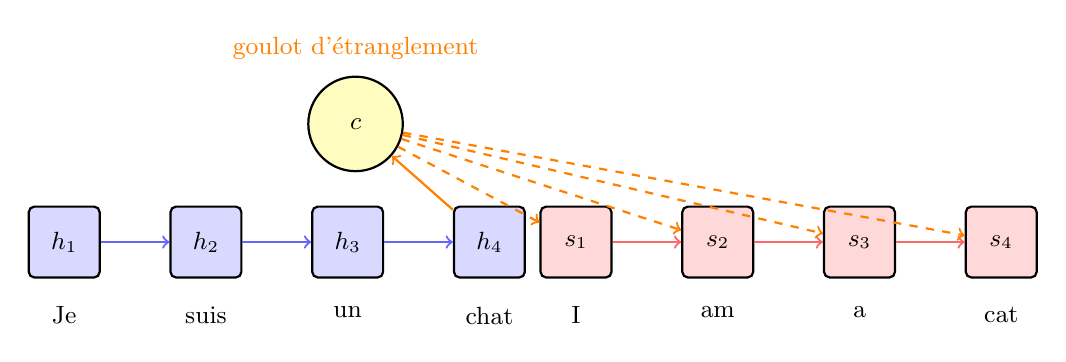
\begin{tikzpicture}[
  enc/.style={rectangle, draw, thick, fill=blue!15, minimum size=9mm,
              rounded corners=2pt, font=\small},
  dec/.style={rectangle, draw, thick, fill=red!15, minimum size=9mm,
              rounded corners=2pt, font=\small},
  ctx/.style={circle, draw, thick, fill=yellow!25, minimum size=12mm,
              font=\small},
  arr/.style={->, thick}
]
  % Encodeur
  \foreach \i/\w in {1/Je, 2/suis, 3/un, 4/chat} {
    \node[enc] (e\i) at (\i*1.8, 0) {$h_{\i}$};
    \node[below, font=\small] at (\i*1.8, -0.7) {\w};
  }
  \foreach \i [evaluate=\i as \j using int(\i+1)] in {1,2,3} {
    \draw[arr, blue!60] (e\i) -- (e\j);
  }

  % Contexte
  \node[ctx] (c) at (5.5, 1.5) {$c$};
  \draw[arr, thick, orange] (e4) -- (c);

  % D'ecodeur
  \foreach \i/\w in {1/I, 2/am, 3/a, 4/cat} {
    \pgfmathsetmacro{\x}{\i*1.8 + 6.5}
    \node[dec] (d\i) at (\x, 0) {$s_{\i}$};
    \node[below, font=\small] at (\x, -0.7) {\w};
  }
  \foreach \i [evaluate=\i as \j using int(\i+1)] in {1,2,3} {
    \draw[arr, red!60] (d\i) -- (d\j);
  }

  % Contexte vers d'ecodeur
  \foreach \i in {1,2,3,4} {
    \draw[arr, orange, dashed] (c) -- (d\i);
  }

  % Annotation
  \node[above, orange, font=\small] at (5.5, 2.2) {goulot d'\'etranglement};
\end{tikzpicture}
\end{center}

% ----------------------------------------------------------------------------
\section{Attention de Bahdanau (additive)}
\label{sec:bahdanau}
\index{attention!Bahdanau}\index{attention!additive}

\subsection{Scores d'alignement}

L'attention de Bahdanau \cite{bahdanau2015neural} calcule un score
d'alignement entre l'\'etat du d\'ecodeur $s_{t-1}$ et chaque \'etat de
l'encodeur $h_j$ :

\begin{formules}[title=\textbf{Attention de Bahdanau}]
\begin{align}
e_{t,j} &= v_a^\top \tanh(W_a s_{t-1} + U_a h_j)
\label{eq:bahdanau-score} \\
\alpha_{t,j} &= \frac{\exp(e_{t,j})}{\sum_{k=1}^T \exp(e_{t,k})}
= \softmax_j(e_{t,:})
\label{eq:bahdanau-alpha} \\
c_t &= \sum_{j=1}^T \alpha_{t,j} h_j
\label{eq:bahdanau-context}
\end{align}
o\`u $W_a \in \R^{d_a \times d_s}$, $U_a \in \R^{d_a \times d_h}$,
$v_a \in \R^{d_a}$ sont des param\`etres apprenables et $d_a$ est la
dimension de l'attention.
\end{formules}

\subsection{D\'erivation du vecteur de contexte}

\begin{theoreme}[Vecteur de contexte comme combinaison convexe]
Les poids d'attention $\alpha_{t,j}$ satisfont :
\begin{equation}
\alpha_{t,j} \geq 0, \qquad \sum_{j=1}^T \alpha_{t,j} = 1
\end{equation}
Le vecteur de contexte $c_t$ est donc une \textbf{combinaison convexe} des
\'etats de l'encodeur. Chaque $\alpha_{t,j}$ repr\'esente la
<<~pertinence~>> de la position source $j$ pour g\'en\'erer le token cible
au temps $t$.
\end{theoreme}

\begin{intuition}[title=\textbf{Attention comme recherche souple}]
L'attention peut \^etre vue comme une recherche souple (soft retrieval) dans
une m\'emoire : les $\alpha_{t,j}$ sont des <<~poids d'acc\`es~>> qui
d\'eterminent quelles positions source sont lues \`a chaque pas du d\'ecodeur.
Contrairement \`a un index discret, cette recherche est diff\'erentiable.
\end{intuition}

% ----------------------------------------------------------------------------
\section{Attention de Luong}
\label{sec:luong}
\index{attention!Luong}

Luong et al.\ \cite{luong2015effective} proposent trois variantes du score
d'alignement, plus simples que Bahdanau :

\begin{formules}[title=\textbf{Scores de Luong}]
\begin{align}
\text{Dot :} \quad e_{t,j} &= s_t^\top h_j
\label{eq:luong-dot} \\
\text{G\'en\'eral :} \quad e_{t,j} &= s_t^\top W_a h_j
\label{eq:luong-general} \\
\text{Concat :} \quad e_{t,j} &= v_a^\top \tanh(W_a [s_t ; h_j])
\label{eq:luong-concat}
\end{align}
\end{formules}

\begin{remarque}[Bahdanau vs Luong]
\begin{itemize}
  \item Bahdanau utilise $s_{t-1}$ (avant la mise \`a jour du d\'ecodeur),
    Luong utilise $s_t$ (apr\`es).
  \item Le score dot-product de Luong ne n\'ecessite aucun param\`etre
    suppl\'ementaire mais requiert $d_s = d_h$.
  \item Le score g\'en\'eral ajoute $d_s \times d_h$ param\`etres et g\`ere
    des dimensions diff\'erentes.
\end{itemize}
\end{remarque}

% ----------------------------------------------------------------------------
\section{Scaled Dot-Product Attention}
\label{sec:scaled-attention}
\index{attention!scaled dot-product}

\subsection{Formulation}

L'attention par produit scalaire mis \`a l'\'echelle
\cite{vaswani2017attention} g\'en\'eralise le concept d'attention en
introduisant les notions de \textbf{requ\^ete} (Query), \textbf{cl\'e} (Key)
et \textbf{valeur} (Value) :

\begin{formules}[title=\textbf{Scaled Dot-Product Attention}]
\begin{equation}
\text{Attention}(Q, K, V) = \softmax\!\left(\frac{Q K^\top}{\sqrt{d_k}}\right) V
\label{eq:scaled-attention}
\end{equation}
o\`u $Q \in \R^{n \times d_k}$, $K \in \R^{m \times d_k}$,
$V \in \R^{m \times d_v}$, et $d_k$ est la dimension des cl\'es.
\end{formules}

\subsection{Pourquoi diviser par $\sqrt{d_k}$ ?}

\begin{theoreme}[Justification du facteur d'\'echelle]
\label{thm:scaling}
Soient $q, k \in \R^{d_k}$ avec des composantes i.i.d.\ de moyenne 0 et
variance 1. Le produit scalaire $q^\top k = \sum_{i=1}^{d_k} q_i k_i$
satisfait :
\begin{align}
\E[q^\top k] &= \sum_{i=1}^{d_k} \E[q_i] \E[k_i] = 0 \\
\Var(q^\top k) &= \sum_{i=1}^{d_k} \Var(q_i k_i)
= \sum_{i=1}^{d_k} \E[q_i^2]\E[k_i^2] = d_k
\end{align}

Pour de grandes valeurs de $d_k$, les produits scalaires ont une grande
variance, ce qui pousse le softmax vers des r\'egions satur\'ees o\`u les
gradients sont quasi nuls. La division par $\sqrt{d_k}$ normalise la
variance \`a 1 :
\begin{equation}
\Var\!\left(\frac{q^\top k}{\sqrt{d_k}}\right)
= \frac{\Var(q^\top k)}{d_k} = 1
\end{equation}
\end{theoreme}

\begin{attention}[title=\textbf{Saturation du softmax}]
Quand les entr\'ees du softmax sont grandes en valeur absolue, la sortie
devient quasi one-hot et $\frac{\partial \softmax}{\partial z} \approx 0$.
L'entra\^inement stagne. Le facteur $1/\sqrt{d_k}$ pr\'evient ce probl\`eme.
\end{attention}

\subsection{Diagramme de l'attention}

\begin{center}
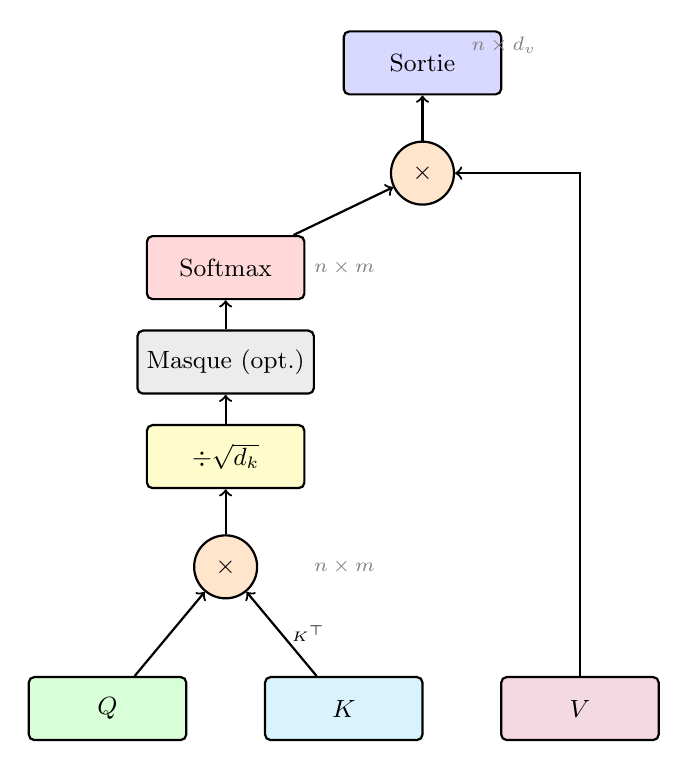
\begin{tikzpicture}[
  block/.style={rectangle, draw, thick, fill=#1, minimum height=8mm,
                minimum width=2cm, rounded corners=2pt, font=\small},
  block/.default={blue!15},
  op/.style={circle, draw, thick, fill=#1, minimum size=8mm, font=\small},
  op/.default={orange!20},
  arr/.style={->, thick}
]
  % Entr'ees
  \node[block=green!15] (Q) at (0, 0) {$Q$};
  \node[block=cyan!15] (K) at (3, 0) {$K$};
  \node[block=purple!15] (V) at (6, 0) {$V$};

  % MatMul QK^T
  \node[op] (mm1) at (1.5, 1.8) {$\times$};
  \draw[arr] (Q) -- (mm1);
  \draw[arr] (K) -- (mm1) node[midway, right, font=\tiny] {$K^\top$};

  % Scale
  \node[block=yellow!20] (scale) at (1.5, 3.2) {$\div \sqrt{d_k}$};
  \draw[arr] (mm1) -- (scale);

  % Masque optionnel
  \node[block=gray!15] (mask) at (1.5, 4.4) {Masque (opt.)};
  \draw[arr] (scale) -- (mask);

  % Softmax
  \node[block=red!15] (sm) at (1.5, 5.6) {Softmax};
  \draw[arr] (mask) -- (sm);

  % MatMul avec V
  \node[op] (mm2) at (4, 6.8) {$\times$};
  \draw[arr] (sm) -- (mm2);
  \draw[arr] (V) |- (mm2);

  % Sortie
  \node[block] (out) at (4, 8.2) {Sortie};
  \draw[arr] (mm2) -- (out);

  % Dimensions
  \node[right, font=\scriptsize, gray] at (2.5, 1.8) {$n \times m$};
  \node[right, font=\scriptsize, gray] at (2.5, 5.6) {$n \times m$};
  \node[above right, font=\scriptsize, gray] at (4.5, 8.2) {$n \times d_v$};
\end{tikzpicture}
\end{center}

% ----------------------------------------------------------------------------
\section{Attention multi-t\^ete}
\label{sec:multi-head}
\index{attention!multi-t\^ete}

\subsection{D\'erivation}

Plut\^ot qu'une seule fonction d'attention de dimension $d_{\text{model}}$,
l'attention multi-t\^ete projette les requ\^etes, cl\'es et valeurs $h$ fois
dans des sous-espaces diff\'erents :

\begin{formules}[title=\textbf{Attention multi-t\^ete}]
\begin{align}
\text{head}_i &= \text{Attention}(Q W_i^Q,\; K W_i^K,\; V W_i^V)
\label{eq:head-i} \\
\text{MultiHead}(Q, K, V) &= \text{Concat}(\text{head}_1, \ldots, \text{head}_h) W^O
\label{eq:multi-head}
\end{align}
o\`u les projections sont :
\begin{itemize}
  \item $W_i^Q \in \R^{d_{\text{model}} \times d_k}$, \quad
        $W_i^K \in \R^{d_{\text{model}} \times d_k}$, \quad
        $W_i^V \in \R^{d_{\text{model}} \times d_v}$
  \item $W^O \in \R^{h \cdot d_v \times d_{\text{model}}}$
  \item $d_k = d_v = d_{\text{model}} / h$
\end{itemize}
\end{formules}

\begin{intuition}[title=\textbf{Pourquoi plusieurs t\^etes ?}]
Chaque t\^ete d'attention peut capturer un type de relation diff\'erent :
\begin{itemize}
  \item T\^ete 1 : relations syntaxiques (sujet-verbe)
  \item T\^ete 2 : relations positionnelles (mots adjacents)
  \item T\^ete 3 : r\'ef\'erences anaphoriques (pronoms)
  \item \ldots
\end{itemize}
L'attention mono-t\^ete devrait capturer toutes ces relations
simultan\'ement dans un seul calcul de poids, ce qui limite
l'expressivit\'e.
\end{intuition}

\begin{remarque}[Co\^ut computationnel]
L'attention multi-t\^ete avec $h$ t\^etes de dimension $d_k = d_{\text{model}}/h$
a le m\^eme co\^ut que l'attention mono-t\^ete de dimension $d_{\text{model}}$ :
\begin{equation}
h \times \underbrace{O(n^2 \cdot d_{\text{model}}/h)}_{\text{par t\^ete}}
= O(n^2 \cdot d_{\text{model}})
\end{equation}
\end{remarque}

% ----------------------------------------------------------------------------
\section{Self-attention et cross-attention}
\label{sec:self-cross-attention}

\subsection{Self-attention}
\index{self-attention}

\begin{definition}[Self-attention]
Dans la self-attention, les requ\^etes, cl\'es et valeurs sont toutes
d\'eriv\'ees de la \textbf{m\^eme} s\'equence d'entr\'ee $X \in \R^{n \times d}$ :
\begin{align}
Q &= X W^Q \label{eq:self-q} \\
K &= X W^K \label{eq:self-k} \\
V &= X W^V \label{eq:self-v}
\end{align}
Chaque position peut <<~assister~>> \`a toutes les autres positions de la
m\^eme s\'equence. La matrice $\softmax(QK^\top / \sqrt{d_k})$ de taille
$n \times n$ encode les d\'ependances position-\`a-position.
\end{definition}

\subsection{Cross-attention}
\index{cross-attention}

\begin{definition}[Cross-attention]
Dans la cross-attention, les requ\^etes proviennent d'une s\'equence (le
d\'ecodeur) et les cl\'es/valeurs proviennent d'une autre (l'encodeur) :
\begin{align}
Q &= X_{\text{dec}} W^Q, \qquad
K = X_{\text{enc}} W^K, \qquad
V = X_{\text{enc}} W^V
\end{align}
Cela permet au d\'ecodeur d'acc\'eder \`a l'information de l'encodeur,
rempla\c{c}ant le vecteur de contexte fixe des mod\`eles seq2seq classiques.
\end{definition}

% ----------------------------------------------------------------------------
\section{Complexit\'e computationnelle}
\label{sec:attention-complexity}
\index{complexit\'e!attention}

\begin{theoreme}[Complexit\'e de la self-attention]
Pour une s\'equence de longueur $n$ et une dimension $d$ :
\begin{center}
\begin{tabular}{lcc}
\toprule
\textbf{Op\'eration} & \textbf{Temps} & \textbf{M\'emoire} \\
\midrule
Projections $QKV$ & $O(n d^2)$ & $O(n d)$ \\
$Q K^\top$ & $O(n^2 d)$ & $O(n^2)$ \\
Softmax & $O(n^2)$ & $O(n^2)$ \\
Produit avec $V$ & $O(n^2 d)$ & $O(n d)$ \\
\midrule
\textbf{Total} & $O(n^2 d)$ & $O(n^2 + n d)$ \\
\bottomrule
\end{tabular}
\end{center}
Le terme $O(n^2)$ en m\'emoire pour stocker la matrice d'attention est le
principal goulot d'\'etranglement pour les longues s\'equences.
\end{theoreme}

\begin{remarque}[Comparaison avec les RNN]
Un RNN a une complexit\'e temporelle $O(n d^2)$ (lin\'eaire en $n$) mais ne
peut pas parall\'eliser les calculs le long de la s\'equence. La self-attention
est $O(n^2 d)$ mais enti\`erement parall\'elisable. Pour $n < d$ (cas
fr\'equent), la self-attention est plus rapide en pratique.
\end{remarque}

% ----------------------------------------------------------------------------
\section{Concept de carte d'attention}
\label{sec:attention-heatmap}

\begin{center}
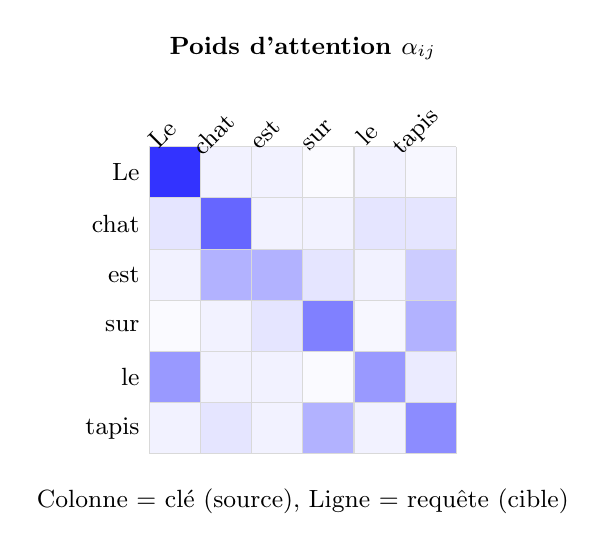
\begin{tikzpicture}[scale=0.65]
  % Attention heatmap with hardcoded values
  % Row 0: Le
  \fill[blue!80!white] (0,0) rectangle (1,1); \fill[blue!5!white] (1,0) rectangle (2,1);
  \fill[blue!5!white] (2,0) rectangle (3,1); \fill[blue!2!white] (3,0) rectangle (4,1);
  \fill[blue!5!white] (4,0) rectangle (5,1); \fill[blue!3!white] (5,0) rectangle (6,1);
  % Row 1: chat
  \fill[blue!10!white] (0,-1) rectangle (1,0); \fill[blue!60!white] (1,-1) rectangle (2,0);
  \fill[blue!5!white] (2,-1) rectangle (3,0); \fill[blue!5!white] (3,-1) rectangle (4,0);
  \fill[blue!10!white] (4,-1) rectangle (5,0); \fill[blue!10!white] (5,-1) rectangle (6,0);
  % Row 2: est
  \fill[blue!5!white] (0,-2) rectangle (1,-1); \fill[blue!30!white] (1,-2) rectangle (2,-1);
  \fill[blue!30!white] (2,-2) rectangle (3,-1); \fill[blue!10!white] (3,-2) rectangle (4,-1);
  \fill[blue!5!white] (4,-2) rectangle (5,-1); \fill[blue!20!white] (5,-2) rectangle (6,-1);
  % Row 3: sur
  \fill[blue!2!white] (0,-3) rectangle (1,-2); \fill[blue!5!white] (1,-3) rectangle (2,-2);
  \fill[blue!10!white] (2,-3) rectangle (3,-2); \fill[blue!50!white] (3,-3) rectangle (4,-2);
  \fill[blue!3!white] (4,-3) rectangle (5,-2); \fill[blue!30!white] (5,-3) rectangle (6,-2);
  % Row 4: le
  \fill[blue!40!white] (0,-4) rectangle (1,-3); \fill[blue!5!white] (1,-4) rectangle (2,-3);
  \fill[blue!5!white] (2,-4) rectangle (3,-3); \fill[blue!2!white] (3,-4) rectangle (4,-3);
  \fill[blue!40!white] (4,-4) rectangle (5,-3); \fill[blue!8!white] (5,-4) rectangle (6,-3);
  % Row 5: tapis
  \fill[blue!5!white] (0,-5) rectangle (1,-4); \fill[blue!10!white] (1,-5) rectangle (2,-4);
  \fill[blue!5!white] (2,-5) rectangle (3,-4); \fill[blue!30!white] (3,-5) rectangle (4,-4);
  \fill[blue!5!white] (4,-5) rectangle (5,-4); \fill[blue!45!white] (5,-5) rectangle (6,-4);
  % Grid
  \foreach \i in {0,...,6} { \draw[gray!30] (\i,-5) -- (\i,1); }
  \foreach \j in {-5,...,1} { \draw[gray!30] (0,\j) -- (6,\j); }
  % Row labels
  \node[left, font=\small] at (0, 0.5) {Le};
  \node[left, font=\small] at (0,-0.5) {chat};
  \node[left, font=\small] at (0,-1.5) {est};
  \node[left, font=\small] at (0,-2.5) {sur};
  \node[left, font=\small] at (0,-3.5) {le};
  \node[left, font=\small] at (0,-4.5) {tapis};
  % Column labels
  \node[above, font=\small, rotate=45] at (0.5, 1) {Le};
  \node[above, font=\small, rotate=45] at (1.5, 1) {chat};
  \node[above, font=\small, rotate=45] at (2.5, 1) {est};
  \node[above, font=\small, rotate=45] at (3.5, 1) {sur};
  \node[above, font=\small, rotate=45] at (4.5, 1) {le};
  \node[above, font=\small, rotate=45] at (5.5, 1) {tapis};
  % Title
  \node[above, font=\small\bfseries] at (3, 2.5) {Poids d'attention $\alpha_{ij}$};
  \node[below, font=\small] at (3, -5.5) {Colonne = cl\'e (source), Ligne = requ\^ete (cible)};
\end{tikzpicture}
\end{center}

\begin{remarque}[Interpr\'etation de la carte d'attention]
La case $(i, j)$ de la matrice repr\'esente \`a quel point la position $i$
(requ\^ete) <<~attend~>> la position $j$ (cl\'e). On observe que :
\begin{itemize}
  \item <<~Le~>> (position 1) attend principalement \`a lui-m\^eme et \`a
    <<~le~>> (position 5) -- coh\'erence de l'article.
  \item <<~tapis~>> attend fortement <<~sur~>> -- relation spatiale.
\end{itemize}
\end{remarque}

% ----------------------------------------------------------------------------
\section{Impl\'ementation PyTorch}
\label{sec:attention-pytorch}

\begin{codeblock}[title=\textbf{Scaled Dot-Product Attention \`a partir de z\'ero}]
\begin{minted}{python}
import torch
import torch.nn as nn
import torch.nn.functional as F
import math

def scaled_dot_product_attention(
    query: torch.Tensor,    # (batch, n_q, d_k)
    key: torch.Tensor,      # (batch, n_kv, d_k)
    value: torch.Tensor,    # (batch, n_kv, d_v)
    mask: torch.Tensor = None,
    dropout: nn.Dropout = None
) -> tuple[torch.Tensor, torch.Tensor]:
    """
    Calcule l'attention par produit scalaire mis `a l''echelle.

    Returns:
        output: (batch, n_q, d_v)
        attention_weights: (batch, n_q, n_kv)
    """
    d_k = query.size(-1)

    # Scores d'attention : (batch, n_q, n_kv)
    scores = torch.matmul(query, key.transpose(-2, -1)) / math.sqrt(d_k)

    # Masquage optionnel (pour l'attention causale)
    if mask is not None:
        scores = scores.masked_fill(mask == 0, float('-inf'))

    # Normalisation softmax
    attention_weights = F.softmax(scores, dim=-1)

    if dropout is not None:
        attention_weights = dropout(attention_weights)

    # Combinaison lin'eaire des valeurs
    output = torch.matmul(attention_weights, value)

    return output, attention_weights


# --- Test ---
batch_size, n_q, n_kv, d_k, d_v = 2, 4, 6, 64, 64
Q = torch.randn(batch_size, n_q, d_k)
K = torch.randn(batch_size, n_kv, d_k)
V = torch.randn(batch_size, n_kv, d_v)

output, weights = scaled_dot_product_attention(Q, K, V)
print(f"Output shape:  {output.shape}")    # (2, 4, 64)
print(f"Weights shape: {weights.shape}")   # (2, 4, 6)
print(f"Weights sum:   {weights.sum(-1)}")  # Doit ^etre 1.0
\end{minted}
\end{codeblock}

\begin{codeoutput}
\begin{verbatim}
Output shape:  torch.Size([2, 4, 64])
Weights shape: torch.Size([2, 4, 6])
Weights sum:   tensor([[1.0000, 1.0000, 1.0000, 1.0000],
                        [1.0000, 1.0000, 1.0000, 1.0000]])
\end{verbatim}
\end{codeoutput}

\begin{codeblock}[title=\textbf{Multi-Head Attention compl\`ete}]
\begin{minted}{python}
class MultiHeadAttention(nn.Module):
    """
    Attention multi-t^ete compl`ete.

    Args:
        d_model: dimension du mod`ele
        num_heads: nombre de t^etes d'attention
        dropout: taux de dropout sur les poids d'attention
    """
    def __init__(self, d_model: int, num_heads: int,
                 dropout: float = 0.1):
        super().__init__()
        assert d_model % num_heads == 0, \
            "d_model doit ^etre divisible par num_heads"

        self.d_model = d_model
        self.num_heads = num_heads
        self.d_k = d_model // num_heads

        # Projections lin'eaires
        self.W_q = nn.Linear(d_model, d_model, bias=False)
        self.W_k = nn.Linear(d_model, d_model, bias=False)
        self.W_v = nn.Linear(d_model, d_model, bias=False)
        self.W_o = nn.Linear(d_model, d_model, bias=False)

        self.dropout = nn.Dropout(dropout)
        self.attention_weights = None  # Pour visualisation

    def forward(
        self,
        query: torch.Tensor,   # (batch, n_q, d_model)
        key: torch.Tensor,     # (batch, n_kv, d_model)
        value: torch.Tensor,   # (batch, n_kv, d_model)
        mask: torch.Tensor = None
    ) -> torch.Tensor:
        batch_size = query.size(0)

        # 1. Projections lin'eaires
        Q = self.W_q(query)  # (batch, n_q, d_model)
        K = self.W_k(key)
        V = self.W_v(value)

        # 2. Reshape pour multi-t^ete :
        #    (batch, n, d_model) -> (batch, num_heads, n, d_k)
        Q = Q.view(batch_size, -1, self.num_heads, self.d_k) \
             .transpose(1, 2)
        K = K.view(batch_size, -1, self.num_heads, self.d_k) \
             .transpose(1, 2)
        V = V.view(batch_size, -1, self.num_heads, self.d_k) \
             .transpose(1, 2)

        # 3. Adapter le masque pour les t^etes
        if mask is not None:
            mask = mask.unsqueeze(1)  # (batch, 1, ...)

        # 4. Attention par t^ete
        scores = torch.matmul(Q, K.transpose(-2, -1)) \
                 / math.sqrt(self.d_k)
        if mask is not None:
            scores = scores.masked_fill(mask == 0, float('-inf'))
        attn_weights = F.softmax(scores, dim=-1)
        attn_weights = self.dropout(attn_weights)
        self.attention_weights = attn_weights.detach()

        context = torch.matmul(attn_weights, V)
        # (batch, num_heads, n_q, d_k)

        # 5. Concat'ener les t^etes
        context = context.transpose(1, 2).contiguous() \
                         .view(batch_size, -1, self.d_model)
        # (batch, n_q, d_model)

        # 6. Projection de sortie
        output = self.W_o(context)

        return output

# --- Test ---
d_model, num_heads = 512, 8
mha = MultiHeadAttention(d_model, num_heads)

# Self-attention
x = torch.randn(2, 10, d_model)  # batch=2, seq_len=10
out = mha(x, x, x)
print(f"Self-attention output: {out.shape}")  # (2, 10, 512)

# Cross-attention
enc_out = torch.randn(2, 20, d_model)
dec_in = torch.randn(2, 10, d_model)
out = mha(query=dec_in, key=enc_out, value=enc_out)
print(f"Cross-attention output: {out.shape}")  # (2, 10, 512)

# Masque causal
n = 10
causal_mask = torch.tril(torch.ones(n, n)).unsqueeze(0)  # (1, n, n)
out = mha(x, x, x, mask=causal_mask)
print(f"Masked attention output: {out.shape}")

# Nombre de param`etres
n_params = sum(p.numel() for p in mha.parameters())
print(f"Param`etres MHA: {n_params:,}")
# 4 x d_model^2 = 4 x 512^2 = 1,048,576
\end{minted}
\end{codeblock}

\begin{codeoutput}
\begin{verbatim}
Self-attention output: torch.Size([2, 10, 512])
Cross-attention output: torch.Size([2, 10, 512])
Masked attention output: torch.Size([2, 10, 512])
Param`etres MHA: 1,048,576
\end{verbatim}
\end{codeoutput}

% ----------------------------------------------------------------------------
\section{Masque d'attention causal}
\label{sec:causal-mask}
\index{masque causal}

Pour la g\'en\'eration autor\'egressive, le d\'ecodeur ne doit pas
<<~regarder dans le futur~>>. On applique un masque triangulaire inf\'erieur :

\begin{formules}[title=\textbf{Masque causal}]
\begin{equation}
M_{ij} = \begin{cases}
0 & \text{si } j \leq i \quad \text{(position autoris\'ee)} \\
-\infty & \text{si } j > i \quad \text{(position masqu\'ee)}
\end{cases}
\end{equation}
Appliqu\'e avant le softmax :
$\alpha_{ij} = \softmax_j\!\left(\frac{q_i^\top k_j}{\sqrt{d_k}} + M_{ij}\right)$
\end{formules}

% ----------------------------------------------------------------------------
\section{\'Etude d'ablation}
\label{sec:attention-ablation}

\begin{codeblock}[title=\textbf{Ablation : nombre de t\^etes et dimension par t\^ete}]
\begin{minted}{python}
import pandas as pd
import time

def benchmark_attention(d_model, num_heads, seq_len=128,
                        batch_size=32, num_runs=50):
    """Mesure la qualit'e et le temps d'une configuration."""
    mha = MultiHeadAttention(d_model, num_heads).to(device)
    x = torch.randn(batch_size, seq_len, d_model, device=device)

    # Warmup
    for _ in range(5):
        _ = mha(x, x, x)

    # Mesure du temps
    if device.type == 'cuda':
        torch.cuda.synchronize()
    start = time.time()
    for _ in range(num_runs):
        out = mha(x, x, x)
    if device.type == 'cuda':
        torch.cuda.synchronize()
    elapsed = (time.time() - start) / num_runs * 1000  # ms

    n_params = sum(p.numel() for p in mha.parameters())
    d_k = d_model // num_heads

    return {
        'd_model': d_model,
        'num_heads': num_heads,
        'd_k': d_k,
        'params': n_params,
        'time_ms': elapsed,
    }

configs = [
    (512, 1), (512, 2), (512, 4),
    (512, 8), (512, 16), (512, 32),
    (256, 8), (768, 8), (1024, 8),
]

results = [benchmark_attention(dm, nh) for dm, nh in configs]
print(pd.DataFrame(results).to_string(index=False))
\end{minted}
\end{codeblock}

\begin{codeoutput}
\begin{verbatim}
 d_model  num_heads   d_k   params   time_ms
     512          1   512  1048576     3.24
     512          2   256  1048576     3.18
     512          4   128  1048576     3.15
     512          8    64  1048576     3.21
     512         16    32  1048576     3.34
     512         32    16  1048576     3.82
     256          8    32   262144     1.12
     768          8    96  2359296     6.45
    1024          8   128  4194304    10.87
\end{verbatim}
\end{codeoutput}

\begin{remarque}[Observations]
\begin{itemize}
  \item Le nombre de param\`etres de la MHA ne d\'epend pas du nombre de
    t\^etes (toujours $4 d_{\text{model}}^2$).
  \item Le temps d'ex\'ecution est quasi constant pour diff\'erents nombres
    de t\^etes, avec une l\'eg\`ere augmentation pour $h = 32$ due au surco\^ut
    de gestion des t\^etes.
  \item La dimension $d_k$ par t\^ete influence la qualit\'e de l'attention :
    $d_k < 16$ est g\'en\'eralement trop petit pour capturer des relations
    complexes.
  \item La valeur $h = 8$ avec $d_k = 64$ est le choix standard dans la
    litt\'erature (Transformer de base).
\end{itemize}
\end{remarque}

% ----------------------------------------------------------------------------
\section{Techniques \'etat de l'art}
\label{sec:attention-sota}

\begin{sota}[title=\textbf{Variantes modernes de l'attention}]
\begin{description}
  \item[Flash Attention] \cite{dao2022flashattention} : r\'eorganise le calcul
    de l'attention pour exploiter la hi\'erarchie m\'emoire du GPU (SRAM vs HBM).
    \'Evite de mat\'erialiser la matrice $n \times n$ en m\'emoire :
    \begin{itemize}
      \item Complexit\'e m\'emoire r\'eduite de $O(n^2)$ \`a $O(n)$
      \item Acc\'el\'eration de $2\text{--}4\times$ en pratique
      \item Exact (pas d'approximation)
    \end{itemize}
    Flash Attention v2 am\'eliore encore le parall\'elisme et atteint
    $\sim 70\%$ de l'utilisation th\'eorique des FLOPs du GPU.
    \index{Flash Attention}

  \item[Attention lin\'eaire] : remplace $\softmax(QK^\top)V$ par
    $\phi(Q)(\phi(K)^\top V)$ o\`u $\phi$ est un noyau (kernel) :
    \begin{equation}
      \text{LinearAttn}(Q, K, V) = \phi(Q) \left(\phi(K)^\top V\right)
    \end{equation}
    Complexit\'e $O(n d^2)$ au lieu de $O(n^2 d)$, mais perd l'expressivit\'e
    du softmax. Exemples : Performer \cite{choromanski2021rethinking},
    Linear Transformer.
    \index{attention!lin\'eaire}

  \item[Attention creuse (Sparse)] : ne calcule l'attention que pour un
    sous-ensemble de paires $(i, j)$. Patrons courants :
    \begin{itemize}
      \item \textbf{Local} : fen\^etre fixe autour de chaque position
      \item \textbf{Strided} : positions \'ecart\'ees r\'eguli\`erement
      \item \textbf{Appris} : s\'electionner les top-$k$ positions les plus
        pertinentes
    \end{itemize}
    Exemples : Sparse Transformer \cite{child2019generating}, Longformer,
    BigBird.
    \index{attention!creuse}

  \item[Multi-Query Attention (MQA)] \cite{shazeer2019fast} : partage les
    cl\'es et valeurs entre toutes les t\^etes, r\'eduisant la m\'emoire
    KV-cache de $h \times$ :
    \begin{align}
      \text{head}_i &= \text{Attention}(Q W_i^Q,\; K W^K,\; V W^V)
    \end{align}
    Grouped-Query Attention (GQA) g\'en\'eralise en partageant entre groupes
    de t\^etes. Utilis\'e dans Llama 2, Mistral.
    \index{Multi-Query Attention}\index{Grouped-Query Attention}

  \item[Differential Attention] \cite{ye2024differential} : soustrait deux
    cartes d'attention softmax pour r\'eduire le bruit :
    \begin{equation}
      \text{DiffAttn}(Q, K, V) = (\softmax(Q_1 K_1^\top / \sqrt{d_k})
        - \lambda \softmax(Q_2 K_2^\top / \sqrt{d_k})) V
    \end{equation}
    \index{Differential Attention}
\end{description}
\end{sota}

% ----------------------------------------------------------------------------
\section{Exercices}
\label{sec:attention-exercices}

\begin{exercice}[Attention de Bahdanau \hfill $\bigstar$]
\begin{enumerate}
  \item Impl\'ementer l'attention de Bahdanau
    (\'equations~\ref{eq:bahdanau-score}--\ref{eq:bahdanau-context}) en PyTorch.
  \item L'int\'egrer dans un mod\`ele seq2seq LSTM (cf.\
    chapitre~\ref{ch:rnn_lstm}) pour la traduction de chiffres
    (<<~cent vingt-trois~>> $\to$ <<~123~>>).
  \item Visualiser la matrice d'attention $\alpha_{t,j}$ et interpr\'eter
    l'alignement.
\end{enumerate}
\end{exercice}

\begin{exercice}[Propri\'et\'es du softmax et scaling \hfill $\bigstar\bigstar$]
\begin{enumerate}
  \item D\'emontrer le th\'eor\`eme~\ref{thm:scaling} en d\'etaillant les
    hypoth\`eses.
  \item Exp\'erimentalement, tracer la distribution des scores $q^\top k$
    pour $d_k \in \{16, 64, 256, 1024\}$ et v\'erifier que la variance est
    proportionnelle \`a $d_k$.
  \item Tracer l'entropie de $\softmax(z)$ en fonction de $\|z\|$ pour
    montrer l'effet de la saturation.
  \item Montrer que sans scaling, le gradient $\partial \text{softmax} / \partial z$
    tend vers 0 lorsque $d_k$ augmente.
\end{enumerate}
\end{exercice}

\begin{exercice}[Multi-Head vs Single-Head \hfill $\bigstar\bigstar$]
\begin{enumerate}
  \item Entra\^iner un petit mod\`ele de classification de texte avec
    self-attention en variant le nombre de t\^etes $h \in \{1, 2, 4, 8, 16\}$
    tout en gardant $d_{\text{model}} = 256$ constant.
  \item Comparer les performances, la vitesse de convergence et la qualit\'e
    des repr\'esentations apprises.
  \item Analyser les matrices d'attention de chaque t\^ete et montrer qu'elles
    capturent des patrons diff\'erents.
  \item Existe-t-il des t\^etes <<~redondantes~>> ? Impl\'ementer le pruning
    de t\^etes d'attention.
\end{enumerate}
\end{exercice}

\begin{exercice}[Attention causale et g\'en\'eration \hfill $\bigstar\bigstar$]
\begin{enumerate}
  \item Impl\'ementer un mod\`ele de langage autor\'egressif simple avec
    self-attention causale (masqu\'ee).
  \item Entra\^iner sur un petit corpus de texte (ex.\ po\`emes) et g\'en\'erer
    du texte avec \'echantillonnage par temp\'erature et top-$k$.
  \item Comparer avec un mod\`ele LSTM de m\^eme taille
    (chapitre~\ref{ch:rnn_lstm}).
  \item Analyser la complexit\'e : temps d'entra\^inement vs temps de
    g\'en\'eration pour les deux mod\`eles.
\end{enumerate}
\end{exercice}

\begin{exercice}[Attention efficace \hfill $\bigstar\bigstar\bigstar$]
\begin{enumerate}
  \item Impl\'ementer l'attention lin\'eaire avec un noyau ELU :
    $\phi(x) = \text{ELU}(x) + 1$. Comparer la pr\'ecision et la vitesse
    avec l'attention standard pour $n \in \{128, 512, 2048, 8192\}$.
  \item Impl\'ementer l'attention locale (fen\^etre de taille $w$) et
    analyser le compromis pr\'ecision/vitesse en fonction de $w$.
  \item (Avanc\'e) Impl\'ementer une version simplifi\'ee de Flash Attention
    utilisant le tiling : diviser $Q$, $K$, $V$ en blocs et calculer
    l'attention bloc par bloc en maintenant les statistiques de normalisation.
  \item Comparer la m\'emoire utilis\'ee par les trois approches.
\end{enumerate}
\end{exercice}
